\documentclass[10pt,twocolumn,letterpaper]{article}

\usepackage{cvpr}
\usepackage{times}
\usepackage{epsfig}
\usepackage{graphicx}
\usepackage{amsmath}
\usepackage{amssymb}
% Include other packages here, before hyperref.
% \usepackage[outdir=./]{epstopdf}

% If you comment hyperref and then uncomment it, you should delete
% egpaper.aux before re-running latex.  (Or just hit 'q' on the first latex
% run, let it finish, and you should be clear).
\usepackage[breaklinks=true,bookmarks=false]{hyperref}

\cvprfinalcopy % *** Uncomment this line for the final submission

\def\cvprPaperID{3510} % *** Enter the CVPR Paper ID here
\def\httilde{\mbox{\tt\raisebox{-.5ex}{\symbol{126}}}}

%% Custom control sequences
\let\oldPr\Pr
\newcommand{\bR}{\mathbb{R}}
\renewcommand*{\Pr}[1]{\mathbb{P}\left( #1 \right)}
\newcommand{\mat}[1]{\mathbf{#1}}
\DeclareMathOperator*{\argmax}{arg\,max}
\DeclareMathOperator*{\argmin}{arg\,min}
\newcommand{\tr}{\mathbf{tr}}
\newcommand{\cross}[1]{[#1]_{\times}}


% Pages are numbered in submission mode, and unnumbered in camera-ready
%\ifcvprfinal\pagestyle{empty}\fi
\setcounter{page}{1}
\begin{document}

%%%%%%%%% TITLE
% \title{All Graphs Lead to Rome: \\
% Cycle Consistent Multi-View Representations Using Graph CNNs}
\title{All Graphs Lead to Rome: Learning Geometric and Cycle-Consistent Representations with Graph Convolutional Networks}

\author{Stephen Phillips, Kostas Daniilidis \\
GRASP Laboratory, University of Pennsylvania\\
{\tt\small \{stephi, kostas\}@seas.upenn.edu}
% For a paper whose authors are all at the same institution,
% omit the following lines up until the closing ``}''.
% Additional authors and addresses can be added with ``\and'',
% just like the second author.
% To save space, use either the email address or home page, not both
% \and
% Second Author\\
% Institution2\\
% First line of institution2 address\\
% {\tt\small secondauthor@i2.org}
}

% When placing figures in \LaTeX, it's almost always best to use
% \verb+\includegraphics+, and to specify the  figure width as a multiple of
% the line width as in the example below
% {\small\begin{verbatim}
%    \usepackage[dvips]{graphicx} ...
%    \includegraphics[width=0.8\linewidth]
%                    {myfile.eps}
% \end{verbatim}
% }


\maketitle
%\thispagestyle{empty}

% Papers, excluding the references section,
% must be no longer than eight pages in length. The references section
%%%%%%%%% ABSTRACT
\begin{abstract}
    Image feature matching is a fundamental part of many geometric computer vision applications, and using multiple images can improve performance.
    In this work, we formulate multi-image matching as a graph embedding problem then use a Graph Neural Network to learn an appropriate embedding function for aligning image features.
    We use cycle consistency to train our network in an unsupervised fashion, since ground truth correspondence is difficult or expensive to acquire.
    In addition, geometric consistency losses can be added at training time, even if the information is not available in the test set, unlike previous approaches which optimize cycle consistency directly.
    To the best of our knowledge, no other works have used learning for multi-image feature matching.
    Our experiments show that our method is competitive with other optimization based approaches.
\end{abstract}

%------------------------------------------------------------------------
\begin{figure}[t]
\begin{center}
  % \fbox{\rule{0pt}{2in} \rule{0.9\linewidth}{0pt}}
  \includegraphics[width=0.9\linewidth]{figures-CycleConsistencyMainFigure-v3.pdf}
\end{center}
  \caption{
    An illustration of the approach of this work.
    The Graph Neural Neural Network (GNN) \cite{battaglia2018relational} takes as input the graph of matches with vertex features and outputs an embedding over the vertices of the graph (represented by different colors in the figure).
    The final embedding is used to construct a pairwise similarity matrix, which we train to be a low dimensional cycle-consistent representation of the graph adjacency matrix.
    We train the network using a reconstruction loss on the similarity matrix with the noisy adjacency matrix, and geometric consistency information, such as epipolar constraints, to provide an unsupervised training method for the model.
  }
\label{fig:pipeline}
% \label{fig:onecol}
\end{figure}

\section{Introduction}
Feature matching is an essential part of Structure from Motion and many geometric computer vision applications.
The goal in multi-image feature matching is to take 2D image locations from three or more images and find which ones correspond to the same point in the 3D scene.
Works such as Wang et al.~\cite{wang2017multi}, have shown improvement in performance by optimizing cycle consistency, i.e. enforcing the pairwise feature matches to be globally consistent.

However, these multi-view consistency algorithms struggle in distributed and robust settings.
Having image features suited for this task would help improve performance, and deep learning has revolutionized how image features are computed \cite{yi2016lift}.
In this paper, we want to leverage the power of deep representations in order to compute feature descriptors that are robust across multiple views.

In this work, we propose to training a Graph Neural Networks (GNNs) to operate directly on the sparse correspondence graph, allowing it to work in a broad class of environments.
To the best of our knowledge this work is the first to apply deep learning to the multi-view feature matching problem.
We use an unsupervised loss - the cycle consistency loss - to train the network, and thus avoiding the difficulty of expensive hand labeling.
Geometric consistency losses can aid training, even if such information is not available at test time.
Although our network is simple, it shows promising results compared to baselines which optimize for cycle-consistency without learned embeddings, using a matrix factorization loss \cite{zhou2015multi, leonardos2016distributed}.
Furthermore, since inference requires only a single forward pass over the neural network, our approach is faster (to achieve comparable accuracy) than methods which must solve an optimization problem every time.
We perform experiments on the Rome16K \cite{li2010location} dataset to test the effectiveness of our method compared to optimization based methods.
% Our contributions in this work are:
% \begin{itemize}
% \item We use a novel architecture to address the multi-image feature matching problem using GNNs with graph embeddings.
% \item We introduce an unsupervised cycle consistency loss that does not require labeled correspondences to train.
% \item We demonstrate the effectiveness of geometric consistency losses in improving training.
% \end{itemize}

\section{Method}
Our goal is to learn optimal features that capture multiple image views by filtering out noisy feature matches.
An outline of our approach can be seen in figure \ref{fig:pipeline}.
We formulate this problem in terms of the correspondence graph of the features.

We assume there is an initial set of feature matches represented as a graph $\mathcal{G} = (\mathcal{V}, \mathcal{E})$, with an associated adjacency matrix $\mat{A}$.
Each vertex of the graph $v \in \mathcal{V}$ is an image feature, corresponding to some ground truth 3D point $\mat{P}(v)$.
Each edge $e = (v_1, v_2) \in \mathcal{E}$ is a potential correspondence.
The graph is constructed from putative correspondences of image features across images, typically constructed using feature descriptor distance (e.g. SIFT feature distance).
Associated with each vertex $v$ is an embedding $\mat{f}_v \in \bR^m$, which can include the visual feature descriptor, position, scale, orientation, etc.
Similarly, each edge $e$ has an associated feature $\mat{f}_e \in \bR^p$ (in this work, initially just the weight of the feature association).
We use these features as the initialization for our learning algorithm.

In the absence of noise or outliers, this graph would have a connected component for each visible point in the world, all mutually disjoint.
Mathematically, this can be expressed as $e = (v_1, v_2) \in \mathcal{E} \implies \mat{P}(v_1) = \mat{P}(v_2)$.
Typically putative correspondences are matched probabilistically, meaning a feature in one image matches to many features in another.
Thus in the noisy case we expect this structure to be corrupted, i.e. there are some edges $e = (v_1, v_2) \in \mathcal{E}$ such that $\mat{P}(v_1) \neq \mat{P}(v_2)$.

While there are many methods for operating on graphs \cite{bronstein2017geometric, bruna2013spectral, defferrard2016convolutional, kipf2017semi, scarselli2009graph, gama2018mimo, gama2018convolutional, battaglia2018relational}
Most of GNNs used in these works can be expressed mathematically as:
\begin{align*}
\mat{\tilde{f}}_v^{(k+1)} =&\; b^{(k)} + \mat{W}_0^{k} \mat{f}_{v}^{(k)} + \sum_{h=0}^H \sum_{v' \in \mathcal{N}^{h}(v)} f_{e(v,v')} \mat{W}_{h}^{k} \mat{f}_{v'}^{(k)} \\
\mat{f}_v^{(k+1)} =&\; \sigma\left(\mat{\tilde{f}}_v^{(k+1)}\right)
\end{align*}
The weights/biases $\mat{W}_{h}^{k}$, $b^{(k)}$ are all learned, with no learning done on the edge weights $f_{e(v,v')}$. 
Note that this is just sums or averages over $h$-hop neighborhoods, where the weights on the edges remain static through the computation.
Given that we are trying to prune edges, it would be sensible to add features over edges to learn which ones to prune and which to keep such as in \cite{scarselli2009graph}.

Therefore, in this work we use the method and implementation described in \cite{battaglia2018relational} (more specifically repetitions of the architecture described in \cite{battaglia2016interaction}).
This work is similar to previous works with one key difference: edges also have weights.
Thus therefore there is intermediate processing on the edges before information is passed to the vertices. 

Mathematically, this is expressed as: % TODO: Maybe make this MLP oriented?
\begin{align}
\mat{\tilde{f}}_{e(v_1,v_2)}^{(k+1)} =&\; \mat{U}_1^{(k)} \mat{f}_{e}^{(k)} + \mat{U}_1^{(k)} \mat{f}_{v_1}^{(k)} + \mat{U}_2^{(k)} \mat{f}_{v_2}^{(k)} \\
\mat{f}_{e(v_1,v_2)}^{(k+1)} =&\; \sigma \left(a^{(k)} + \mat{\tilde{f}}_{e(v_1,v_2)}^{(k+1)}\right) \\
\mat{\tilde{f}}_{v}^{(k+1)} =&\; \mat{W}_0^{(k)} \mat{f}_{v}^{(k)} + \sum_{e \in \mathcal{E}(v)} \mat{W}_1^{(k)} \mat{f}_{e}^{(k+1)} \\
\mat{f}_v^{(k+1)} =&\; \sigma\left(b^{(k)} + \mat{\tilde{f}}_v^{(k+1)}\right)
\end{align}
Here the learned weights are denoted $\mat{W}$ and $\mat{U}$, and the biases $a^{(k)}$ and  $b^{(k)}$.
In \cite{battaglia2018relational}, they allow for more sophisticated aggregation functions, but in this work we simply use the mean function.
In practice, we use MLPs in message passes between vertices and edges for better expressiveness

\subsection{Cycle Consistency}

Let $\mat{M}$ be the noiseless set of matches between our features, with $\mat{M}_{ij}$ being the matches between image $i$ and image $j$.
If the pairwise matches are globally consistent, then we can say that, for all $i, j, k$:
\begin{equation}
\mat{M}_{ij} = \mat{M}_{ik} \mat{M}_{kj}
\label{eq:cycconsist1}
\end{equation}
In other words, the matches between two images stay the same no matter what path is taken to get there. 
This constraint is known as \textit{cycle consistency}, and has been used in a number of works to optimize for global consistency \cite{zhou2015multi, wang2017multi, leonardos2016distributed}.
Stated in this form, there are $O(n^3)$ cycle consistency constraints to check.
A more elegant way to represent cycle consistency is to first create a `universe' of features that all images match to.
Then, one can match the $i^{th}$ set of features to the universe using a ground-truth matching matrix $\mat{X}_i$.
Then the cycle consistency constraint becomes:
\begin{equation}
\mat{M}_{ij} = \mat{X}_{i}\mat{X}_{j}^\top
\label{eq:cycconsist2}
\end{equation}

This reduces the number of our constraints from $O(n^3)$ to $O(n^2)$.
We try to learn vertex embeddings $\mat{F}_V$ to approximate $\mat{X}$ - in other words the final embedding should be an encoding of the universe of features.
As we do not have the ground truth matches $\mat{M}$, we approximate it using the noisy adjacency matrix $\mat{A}$ of our correspondence graph. Thus our loss would be 
\begin{equation}
\mathcal{L}(\mat{A}, \mat{F}_V) = \mathcal{D}(\mat{A}, \mat{F}_V \mat{F}_V^\top)
\end{equation}
Here $\mathcal{D}$ could be an $L_2$ loss, $L_1$ loss, or many others. In this work, we use the $L_1$ loss. 

\subsection{Geometric Consistency Loss}

One of the main advantages of this approach over more traditional optimization based approaches is the ability to add geometric consistency information into the loss at training time, even if it is not available at test time.
The simplest way to add geometric consistency losses, and the approach we use here, is to use the epipolar constraint.
The epipolar constraint describes how the positions of features in different images corresponding to the same point should be related.
The epipolar constraint between two cameras $i$ and $j$  (transforms $j$ to $i$) on corresponding feature locations $X_{i,k}$ and $X_{j,l}$ is (derived in \cite{tron2014quotient}):
\begin{equation}
X_{i,k}^\top R_{i}^\top \cross{T_{j} - T_{i}}R_{j} X_{j,l} = 0
\label{eq:essential_constraint}
\end{equation}
The constraint assumes that the $X_k$ are calibrated (i.e. the camera intrinsics are known). 
Given our vertex embeddings matrix $\mat{F}_V$, we can formulate a loss between all cameras $i$ and $j$:
\begin{align} 
\mathcal{L}_{geom}(\mat{F}_V)
=&\; \mathrm{tr}(\mat{G}^\top \mat{F}_V\mat{F}_V^\top) = \sum_{k,l} (\mat{F}_V)_{k} \cdot (\mat{F}_V)_{l} (\mat{G})_{kl} \label{eq:geom_cost2} \\
(\mat{G})_{kl} =&\; \left|X_{k}^\top R_{c(k)}^\top \cross{T_{c(l)} - T_{c(k)}}R_{c(l)} X_{l}\right| \nonumber
\end{align}
Where $c(k)$ is the appropriate camera for point index $k$.




\begin{figure*}[t]
\begin{center}
  % \fbox{\rule{0pt}{2in} \rule{.9\linewidth}{0pt}}
  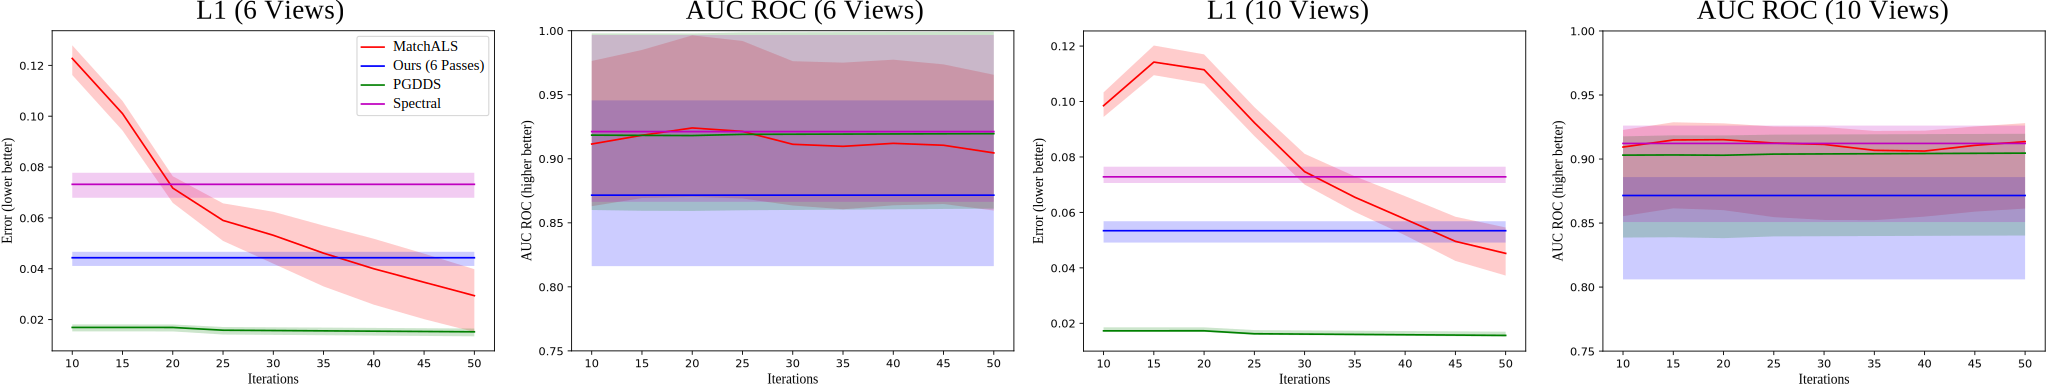
\includegraphics[width=0.95\linewidth]{figures-error_lines-v2.pdf}
  \end{center}
     \caption{
         Plot of the losses of the baselines at different iteration numbers.
         The line shows the mean of the graph while the translucent coloring shows the $25^{th}$ to $75^{th}$ percentiles.
         The ROC AUC curves remain fairly consistent while the L1 loss goes noticibly down after more iterations.
         Our method compares to 35-45 iterations of MatchALS, while only having 16 layers and 8 message passes.
         PGDDS performs better than us in $L_1$ but we perform similarly in the ROC AUC metric.
     }
  % \label{fig:twocol}
  \label{fig:errorlines}
\end{figure*}


\subsubsection*{Acknowledgements}
Support by ARL DCIST CRA W911NF-17-2-0181, NSF-IIS-1703319, ARL RCTA W911NF-10-2-0016, ONR N00014-17-1-2093, and the Honda Research Institute is gratefully acknowledged.

{\small
\bibliographystyle{ieee}
\bibliography{egbib}
}


\end{document}
